\documentclass{article}
\usepackage{graphicx} % Required for inserting images

\title{Bayard Walsh Algorithms Midterm}
\author{Bayard Walsh}
\date{February 2023}

\begin{document}

\maketitle

\section{Question 1: Hopping Game}
Solution: \newline 
\textbf{Input:} A sequence of $n+1$ positions, where some of the positions $j$ in the range $1$ to $n-1$ have an obstacle.\newline\newline
\textbf{Desired Output:} the minimum number of moves required to win the game (or “can’t win” if it’s impossible)  \newline \newline
\textbf{General Approach:} Create an array of length $n$, where every index represents the minimum steps needed to reach index $n$ from $0$, which is our start point. The array will function similar to a Dijkstra path. Set every value to $\infty$ to start, and then set $d[0]=0$, because the first index represents the starting position. Starting from $i=0$ and looping forwards, we first check if $A[i]$ is an obstacle. If so, $A[i]$ is always unreachable, so we leave as $\infty$. If not, we have $p=d[i]$, or we record the minimum steps to reach $d[i]$ from $0$. Then we consider the positions $i+1,i+2,i+3,i+4$ represented as $k$, or the positions that we could reach from taking $1,2,3,$ or $4$ steps from $i$. For a given position $k$, if $A[k]$ is an obstacle, we leave as $\infty$, because it is unreachable. If it is not an obstacle, we update it to be the min of $d[k]$ and $p+1$ (shortest path to $d[i]$ plus one step). If uninitialized, it will always be $p+1$, because values are first set to $\infty$, so $min=p+1$. If not, we take the min, because there may be many paths to reach a certain position $k$ and we only want the shortest one in $d[k]$. We repeat this approach for every $4$ values ahead of $i$ for every $i$, and gradually build an array $d[]$ so that any given value $i \in \{1, 2 \cdots n \}$ is either $\infty$ if unreachable, or $d[i]$ which is the shortest path from the start at a given step. We then check the last value, which will be the min steps to the end, if it is possible. If $M_p= \infty$, we know that there is no possible path. \newline \newline
\textbf{Algorithm($A[1, 2 \cdots n-1 ]$)} \textit{// array of positions indicating obstacle}\newline
 if $n \leq 4$ \textit{ // edge case checking } \newline 
\indent \textbf{return 1} \newline 
 $d[n]= \infty$ \textit{// create $n$ sized array for min steps to position array, all positions $\{0,1, 2 \cdots n-1 \}$ $\in d[]$ initialized to $\infty$. Note the $0$ index is for starting spot} \newline\newline
 $d[0]=0$ \textit{// \textbf{NOTE:} Set  $d[0]$to $0$} \newline
 $i=0$ \textit{// Starts at $0$} \newline
 while $i <n$ \textbf{do:} \newline
 \indent if ($A[i] \neq 1$ \textbf{do:} \newline
 %\textit{// if $A[i] = 1$, then $i$ is an obstacle, so no paths to $i$ are valid. if $d[i] = \infty$ then the path hasn't been updated by a position ahead of it. As we are going backwards, this also means that no paths through $i$ can reach the end. As $i=n$ will be invalid for $A[n]$, we add $i \neq n$ to make sure we have this step } \newline \newline 
 \indent\indent $k=i+1$ \textit{// check values in front of $i$} \newline
 \indent\indent $p=d[i]$ \textit{// minimum steps to reach $i$} \newline 
\indent \indent  while $k\leq i+4$ \textbf{AND} $k < n$ \textbf{do:} \newline  
\indent \indent \indent \textit{// checks each of the $4$ spots in front of $i$, and $k < n$ so no outside indexing} \newline
 \indent\indent \indent if $A[k] \neq 1$ \textbf{do:} \textit{// check for obstacle, if no obstacle, possible path} \newline
%\indent \indent \indent \indent if $A[k] \neq -1$ \textbf{do:} \textit{// check if uninitialized} \newline
% \indent \indent \indent \indent \indent $A[k] = p+1$ \textit{// if create  path to end} \newline
% \indent \indent \indent \indent \textbf{else:} \newline
\indent  \indent \indent \indent \indent $d[k] = min\{d[k],p+1\}$ \textit{// update min steps to $d[k]$. Only change if shorter} \newline \newline 
\indent \indent \indent $k=k+1$ \textit{ // increment $k$} \newline \newline 
\indent $i=i+1$ \textit{ // increment $i$}\newline 
$M_p=min\{d[n-4],d[n-3],d[n-2],d[n-1]\}$ \textit{ // min value of paths one step from end} \newline
$M_p=M_p+1$ \textit{// one more step required to reach $n$} \newline
if $M_p \neq \infty$ \textbf{do:} \textit{//check if a path is possible} \newline 
\indent \textbf{return $M_p$} \newline 
\textbf{else:} \textit{//if no paths from $\{d[n-4],d[n-3],d[n-2],d[n-1]\}$, no paths are possible} \newline 
\indent \textbf{return “can’t win”} \newline\newline
\textbf{Run time:} In terms of Run time analysis, the algorithm performs in $O(n)$. First it initializes an array of length $n$, setting all values to $\infty$. This is $O(n)$. Second, as it makes one pass through $A[1, 2 \cdots n-1 ]$ in the while loop, from the start of the loop to the end. While there is a nested while loop, this performs a maximum of $4$ steps per $i$ iteration, to check the potential steps forward from $i$. Inside the loop there are constant operations, such as updating the distance value and increasing the while loop counters. Therefore, we can consider the loop to have $O(4n)$ run time, simplifying to $O(n)$. After the loop, we take the minimum values from the last $4$ positions and add one (each is within one step from end), to find the best path, and min is semi-constant operation. Finally, we check for infinity and either return $M_p$ or impossible. Therefore, we have $O(n)+O(4N)$ which simplifies to $O(n)$. \newline\newline
\textbf{Correctness:} \newline
\textbf{Feasibility:} In terms of feasibility, we prove two aspects: \newline
\textbf{First: the algorithm will always return a path if a path is possible} \newline 
\textbf{Proof:} Because the algorithm begins with $d[0]=0$, and builds paths forwards, any position that can be reached from the start will be updated with a non $\infty$ amount, because the loop checks each of the $4$ values in front of every valid index (a valid index is reachable from index $0$) and adds them if they are non-obstacles. Therefore, because any valid path must move at within $1-4$ values ahead of another valid position, the algorithm will incrementally do this, and if there is a valid path eventually then it will be added to $min\{d[n-4],d[n-3],d[n-2],d[n-1]\}$ and returned by the algorithm. Note if any of $\{d[n-4],d[n-3],d[n-2],d[n-1]\}$ $\neq \infty$, a path is possible. \newline
\textbf{Second: the algorithm will never return a path if a path is impossible}\newline \textbf{Proof:} If there is not a valid path from the start to the end, then there must be some point where you cannot move $1,2,3$ or $4$ steps from a valid position, say $p$ towards another valid position on the path to $n$. If this is the case, then when the algorithm arrives at $p$ it will check the $1,2,3$ or $4$ steps ahead, and if none are valid then it will not update any steps. Therefore, all the values after $p$ will equal $\infty$, which will \textbf{return “can’t win”}. \newline
Therefore the algorithm will always always return a path if possible and won't if impossible. \newline\newline
\textbf{Optimality:} 
First, \textbf{Lemma:} \textbf{For each $u \in A[1, 2 \cdots n-1 ]$, $d[u]$ is the length of the fewest steps from $0$ (the starting point) to $u$} \newline 
Proof by induction. If $n \not >4$, we return $1$ by edge case checking. Therefore, our base case is $n=5$, in which case $d[u]=1$ for each $\{d[1],d[2],d[3],d[4]\}$ that doesn't have an obstacle, and $2$ for overall min steps to $n$, which is optimal, meaning that $d[u]$ has offered the fewest steps from $0$ for each $\{d[1],d[2],d[3],d[4]\}$. \newline
\textbf{Induction:} Now suppose this holds for $n \geq 5$. Let $v$ be an arbitrary position which the algorithm has iterated over. Let $p$ be the move-sequence made by the algorithm to reach $v$, such that $|p|=d[u]$. Let $p'$ be any other move-sequence to reach $v$. We want to show that $p'$ cannot be shorter than $p$. Let $u$ be the position of the last move made by both $p$ and $p'$ before the paths diverge. Therefore, let $p$ go to some position $x$ and $p'$ go to some other position $y$, both which are reachable from $u$. However, as the algorithm records every possible move for a given index (it checks each of the $4$ spaces ahead for any given $i$ in the array), the algorithm will either record this step $p'$ in $d[y]$ or $d[y]$ will contain a count of a shorter path to $y$. At the next step of $p'$, at position $y$ the algorithm will once again consider all valid possible moves from $y$. Therefore, for every step $s$ in $p'$, the algorithm will have a path, $d[s] \leq |p'_s|$ where $p'_s$ is the number of steps to reach $s$ given by $p'$. Finally, at some point $p'$ will reach $v$, meaning that it is within $4$ positions of some other valid position. As the algorithm loops through every position, then it will also consider this position, meaning it will consider path $p'$, so $d[v]=min\{|p|,|p'|\}$,and as $|p|=d[u]$, $|p \not > p'|$. Therefore, $|p'|$ is not shorter than $d[v]$, meaning that for any arbitrary $u \in d[u]$, the distance to $d[u]$ is the length of the fewest steps from $0$.\newline
%Let $u$ be the move selected by the algorithm directly before moving to $v$. By assumption, we have $d[u]$ is the minimum amount of steps to reach $u$ and we subsequently have $d[u]+1=d[v]$. Since $u$ has been iterated over, and by assumption, $d[u]$ is the length of the fewest steps from $0$ to $u$ from any path, so there is a path from the start to $v$ which takes $d[u]+1$ steps from $0$ to $v$. We want to show this is the shortest path from $0$ to $v$. \newline
%Consider some other path $P$ from $0$ to $v$ and let $x$ be the first value of $P$ that takes a different path than the one given by the algorithm. 
%Therefore, it steps to a different position than the one given by the algorithm along the way to $v$, say it goes to position $y$ directly after $x$. Consider the amount of steps needed from $0$ to $y$. By inductive hypothesis, this is $d[x]+1$. And by definition of always choosing the fewest steps in our minimization step, we have $d[y] \leq d[x] +1$. However, as the path to $v$ through $u$ was picked by the algorithm, because of it has the fewest steps, then we have $d[v] \leq d[y]$. Therefore, $P$ is not shorter than $d[v]$ \newline
\textbf{Proof: The Algorithm Provides the Fewest Steps to $n$ if a path is possible}. As proven by the previous lemma, for each $u \in A[1, 2 \cdots n-1 ]$, $d[u]$ is the length of the fewest steps from $0$ (the starting point) to $u$. Therefore, consider the paths $d[n-4],d[n-3],d[n-2],d[n-1]$. Note that each of these paths is exactly one step away from $n$, and that these are the only paths that can reach $n$ in one step. Secondly, as each of these values are the minimum paths to the positions $n-4,n-3,n-2,n-1$, and any valid path must go through one of these $4$ positions to reach $n$. Therefore the minimum path must go through at least one of these positions. Therefore, if we taken the $min\{d[n-4],d[n-3],d[n-2],d[n-1]\}$, and add $1$ (each path is equally $1$ step away, so it will still minimize), we will find our shortest path possible to $n$. However, if the $min= \infty$, we know that it wasn't possible to reach any of these positions from $0$, or the start, and as we iterated through the entire array, we know that there cannot be any possible paths to $n$, so we \textbf{return “can’t win”}. \newline
\section{Question 2: MST with one modified edge}
\textbf{Note: I used $e_*$ instead of $e^*$. In regards to any work on the problem $e_*=e^*$. Thanks!} \newline \newline
First, we know that $T$ is the only MST for $w$, because the edges are distinct. Second, we know that $T'$ is the only MST for $w'$ because edges are also distinct. I will show that at its largest $k=1$, after moving from $w$ to $w'$. \newline\newline
\textbf{First case: We will assume that $e_* \in T$.} \newline 
Most of the work on this proof will involving picking another edge $e'$ in the same cutset as $e_*$. This process will be detailed below and I will refer to the same $e'$ and $e_*$ throughout the first case analysis of the proof. Note that picking the \textbf{min} $e'$ in the cut set and $\not\in T$ is the best option for exchange for $e_*$, because if $e'$ can't be exchanged into the MST for $e_*$, a greater value $\not \in$ $G$ couldn't be either.\newline
\textbf{Lemma:} \textit{For $G=(V,E)$ let $S \subseteq V$ be a cut and let $e_*$ and $e'$ be two edges in the cutset $S$, such that $e_* \in T$ and $e' \not\in T$. Pick $e'$ such that $w(e')$ is minimized over all edges that are both in the cutset $S$ and $\not\in T$. Let $C$ be the cycle created by adding $e'$. Then $ (\forall e \in C\setminus e') w(e)< w(e') $}\newline 
First, consider adding $e'(u,v)$ to $T$ while we have the original weights $w$. As adding any edge to $T$ will create a cycle, by its MST property, and we know all weights in $w$ and $w'$ are distinct positive integers, so therefore adding $e'$ will create a cycle $C$ between vertexes $(u,v)$. Therefore, we apply the Cycle Property, implying that the highest-weighted edge in $C$ does not appear in any MST for $G$. As $e'(u,v)$ does not appear in $T$, we know that it must be the highest-weighted edge in $C$, or else the Cycle Property would not hold, implying $T$ is not an MST, a contradiction. Therefore, where $P$ is the path from $(u,v)$ in $T$, $ (\forall w(e) \in P) < w(e')$, and subsequently $ (\forall w(e) \in C \setminus e') < w(e')$ \newline \newline 
\textbf{Lemma:} \textit{For $G=(V,E)$ let $S \subseteq V$ be a cut and let $e_*$ and $e'$ be two edges in the cutset $S$, such that $e_* \in T$ and $e' \not\in T$. Pick $e'$ such that $w(e')$ is minimized over all edges that are both in the cutset $S$ and $\not\in T$. If $w'(e_*)<w'(e')$ then $|T-T'| = 0$}\newline 
As we use the same constraints to pick an $e'$ from the previous lemma, we will regard the same cycle $C$ created above, but with the new weight function $w'$. We will also consider the same path $P$. As $(\forall e \in P) w(e)< w(e')$, and $w(e)=w'(e)$ for all $e\neq e_*$, we know that $(\forall e \in P \setminus e_*) w'(e)< w'(e')$. If we have $w'(e_*)<w'(e')$, we have $ (\forall e \in C \setminus e') w'(e)< w'(e') $, meaning that $e'$ would be the maximum value in a cycle $C$, so $e'$ could not be in any MST, meaning that we have $|T-T'| = 0$ because we can't make any exchanges. \newline \newline
\textbf{Lemma:} \textit{For $G=(V,E)$ let $S \subseteq V$ be a cut and let $e_*$ and $e'$ be two edges in the cutset $S$, such that $e_* \in T$ and $e' \not\in T$. Pick $e'$ such that $w(e')$ is minimized over all edges that are both in the cutset $S$ and $\not\in T$. If $w'(e_*)>w'(e')$ then $|T-T'| \geq 1$}\newline
As we use the same constraints to pick an $e'$ from the previous lemma, we will regard the same cycle $C$ created above, but with the new weight function $w'$. We will also consider the same path $P$. If we have $w'(e_*)>w'(e')$, and we as know that $(\forall e \in P \setminus e_*) w'(e)< w'(e')$, then when we create cycle $C$ which contains path $P$ by adding $e'$, we have $(\forall e \in C) w'(e)< w'(e_*)$. Therefore, we apply the cycle property, and as $w'(e_*)$ is the max value in the cycle $C$, it cannot be in any MST. Therefore, we have $|T-T'| = 1$ in this exchange, as $e_*$ is no longer $\in T$, but it is $\in T'$ \newline \newline 
\textbf{Second case: We will assume that $e_* \not\in T$, to cover all cases.} \newline 
Most of the work on this proof will involving picking another edge $e'$ in the same cutset as $e_*$. This process will be detailed below and I will refer to the same $e'$ and $e_*$ throughout the second case analysis of the proof. Note that picking the \textbf{max} $e'$ in the cut set and $\in T$ is the best option for exchange for $e_*$, because if $e'$ can't be taken out of the MST, a lower edge $\in$ $T$ and in the cutset couldn't be either. \newline
\textbf{Lemma:} \textit{For $G=(V,E)$ let $S \subseteq V$ be a cut and let $e_*$ and $e'$ be two edges in the cutset $S$, such that $e_* \not\in T$ and $e' \in T$. Pick $e'$ such that $w(e')$ is maximized over all edges that are both in the cutset $S$ and $\in T$. Let $C$ be the cycle created by adding $e_*$. Then $ (\forall e \in C \setminus e_*) w(e)< w(e_*) $}\newline 
First, consider adding $e_*(u,v)$ to $T$ while we have the original weights $w$. As adding any edge to $T$ will create a cycle, by its MST property, and we know all weights in $w$ and $w'$ are distinct positive integers, so therefore adding $e_*$ will create a cycle $C$ between vertexes $(u,v)$. Therefore, we apply the Cycle Property, implying that the highest-weighted edge in $C$ does not appear in any MST for $G$. As $e_*(u,v)$ does not appear in $T$, we know that it must be the highest-weighted edge in $C$, or else the Cycle Property would not hold, implying $T$ is not an MST, a contradiction. Therefore, where $P$ is the path from $(u,v)$ in $T$, $ (\forall w(e) \in P) < w(e_*)$, and subsequently $ (\forall w(e) \in C \setminus e_*) < w(e_*)$ \newline \newline 
\textbf{Lemma:} \textit{For $G=(V,E)$ let $S \subseteq V$ be a cut and let $e_*$ and $e'$ be two edges in the cutset $S$, such that $e_* \not\in T$ and $e' \in T$. If $w'(e_*)>w'(e')$ then $|T-T'| = 0$}\newline 
As we use the same constraints to pick an $e'$ from the previous lemma, we will regard the same cycle $C$ created above, but with the new weight function $w'$. We will also consider the same path $P$. As $e'$ is the maximum value in the cutset $\in T$, when we add $e_*$ to create a cycle, if $w'(e_*)>w'(e')$, $w'(e')$ is a smaller edge, meaning adding $e_*$ would be a violation of the MST property. Therefore we add no edges and have $|T-T'| = 0$. \newline \newline
\textbf{Lemma:} \textit{For $G=(V,E)$ let $S \subseteq V$ be a cut and let $e_*$ and $e'$ be two edges in the cutset $S$, such that $e_* \not\in T$ and $e' \in T$. Pick $e'$ such that $w(e')$ is maximized over all edges that are both in the cutset $S$ and $\in T$. If $w'(e_*)>w'(e')$ then $|T-T'| \geq 1$}\newline
As we use the same constraints to pick an $e'$ from the previous lemma, we will regard the same cycle $C$ created above, but with the new weight function $w'$. We will also consider the same path $P$. If we have $w'(e_*)>w'(e')$, and we as know that when we add $e_*$ to create a cycle $\in T$, if $w'(e')> w'(e_*)$, then $w'(e_*)$ is a smaller edge, meaning exchanging $e'$ for $e_*$ will maintain MST property. Therefore we add $e_*$ and we have $|T-T'| = 1$ in this exchange, as $e'$ is no longer $\in T$, but it is $\in T'$ \newline \newline
\textbf{Now we consider if we can reach a greater $|T-T'|$ outside exhanging $e_*$} \newline 
\textbf{Lemma:} \textit{For $G=(V,E)$ let $S \subseteq V$ be a cut and let $e_*$ and $e'$ be two edges in the cutset $S$, such that either $e_* \in T$ and $e' \not\in T$ \textbf{OR} $e_* \not\in T$ and $e' \in T$. Therefore, both $e'$ and $e_*$ bridge the same two connected sub-graphs.}\newline
By definition of a cut, we know that it is a partition of vertices into two nonempty subsets, $(S,V-S)$, where a cut set of $S$ is the set of edges with has exactly one endpoint in $S$. Therefore, when considering that $e'$ and $e_*$ are in the same cut set (which is the only way to exchange one edge from outside and MST into a MST and maintain the MST properties), both $e'$ and $e_*$ have one edge in $S$ and one edge in $V-S$. As we know that $T$ is a minimum spanning tree, we know that \newline \textbf{1}: the only paths between the vertices in $S$ to any in $V-S$ is through whichever edge is $\in T$ for $T$, or else we would have a loop, violating the spanning tree property \newline \textbf{2}: all the nodes in $S$ are connected to each other in some subgraph and that all the nodes in $V-S$ are also a connected to each other in some subgraph, by the spanning tree property. In other words, whichever edge is $\in T$ for $T$ is a bridge between two connected components. \newline
Therefore, let $A$ be a connected sub graph of nodes in $S$ and let $B$ be a connected sub graph of nodes in $V-S$. If neither $e'$ nor $e_*$ is  $ \in T'$, we would have two connected components $A$ and $B$. As we know that all weights are the same except $e_*$ from $w$ to $w'$, and we are weighing either $e_*$ or $e'$ in the MST, then $A$ and $B$ must also be components of $T'$ bridged by either $e_*$ or $e'$. If not, this would imply that there must be some other edge $e_i\neq e_*$ and $e_i\neq e'$ $\in T'$ and $e_i \not \in T$. However, as none of the other weights are changed, then $e_i$ could only be greater than some other edge it would replace in $T$ or else it would violate the MST rules for $T$. If $e_i$ is greater, than it will not be in $T'$, as that would violate the MST rules for $T'$, because the weights haven't changed. Therefore the same two connected components must be in $T$ and $T'$. \newline  
\textbf{Proof:} \textit{At it's largest, $|T-T'|=k=1$} \newline
As proved above, $e'$ and $e_*$ both bridge the same two connected components for $T$ and $T'$. Therefore, the only differences between the two MSTs is if $e_*$ is removed from or added to $T'$ from $T$, as shown in the case analysis above, causing a maximum difference of $1$. Adding any other edge to $T'$ would be a violation of MST attributes. \newline
\textbf{Example Below} \newline
\newline 
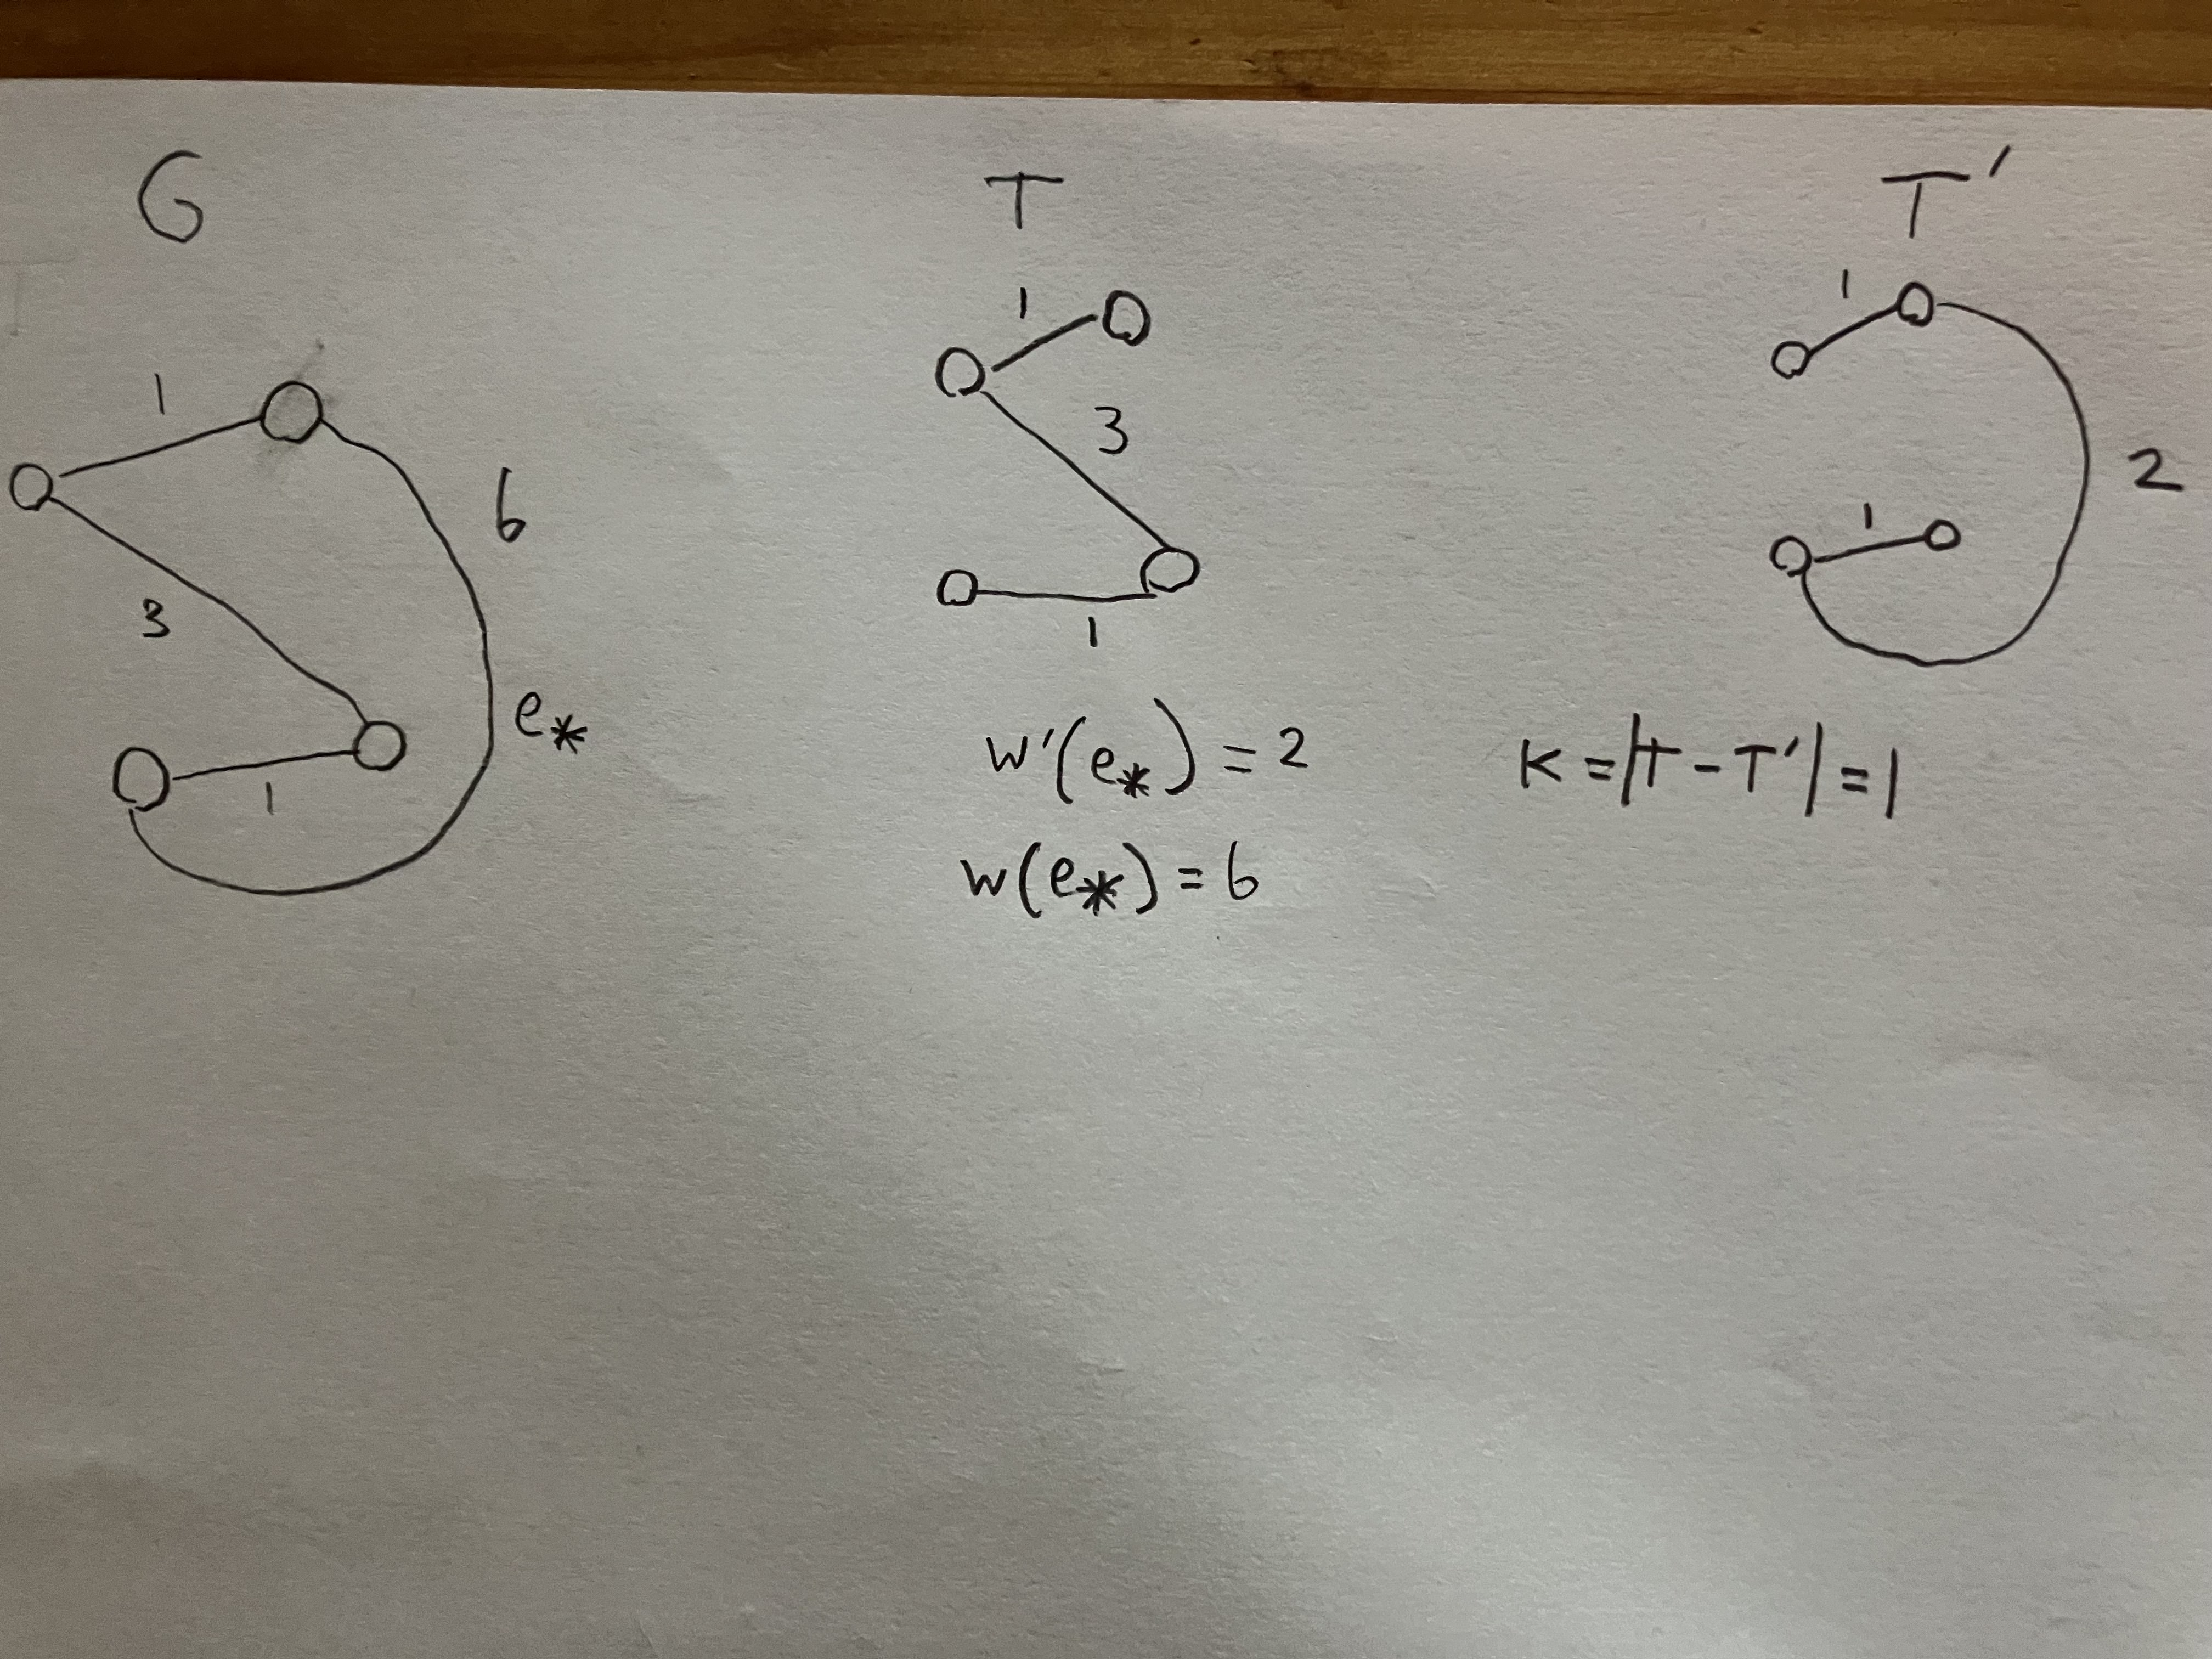
\includegraphics[width=12cm]{IMG_1076}




%\textbf{Lemma:} \textit{If $w(e_*)>'w(e_*)$ and $e_* \in T$ then $|T-T'| = 0$} \newline Let $e_*$ be the edge changed by $w'$ be some arbitrary edge $\in T$, (where $T\subseteq E$ is an MST for $G$). As $e_*$ is changed by $w'$, we know that $w(e_*)<w'(e_*)$ or $w(e_*)>w'(e_*)$. However, if $w(e_*)>w'(e_*)$ and $e_* \in T$, then $w'$ would have reduced the value of an edge already in an MST. As all other values are left unchanged by $w'$, $T$ would still be a spanning tree of $G$ which minimizes the edge weights. Therefore,  $e_*$ would still be an edge in $T'$, and as $T$ would also be an MST for weights $w'$,  $|T-T'| = 0$. \newline \newline

%\textbf{Lemma:} \textit{Picking $e'$ such that $w(e')$ is minimized over all edges that are both in an arbitrary cutset $S$ and $\not\in T$ is equivalent to picking an $e'$ that minimizes all edges that are both in an arbitrary cutset $S$ and $\not\in T$ for $w'(e')$.} \newline 
%As $e' \not \in T$, we know that $e' \neq e_*$. Therefore $ (\forall e' w(e')=w'(e') $, so minimizing for $w$ also minimizes for $w'$. \newline\newline




%\textbf{Lemma:} \textit{If $w(e_*)<'w(e_*)$ and $e_* \not\in T$ then $|T-T'| = 0$} \newline Let $e_*$ be the edge changed by $w'$ be some arbitrary edge $ \not \in T$, (where $T\subseteq E$ is an MST for $G$). As $e_*$ is changed by $w'$, we know that $w(e_*)<w'(e_*)$ or $w(e_*)>w'(e_*)$. However, if $w(e_*)<w'(e_*)$ and $e_* \not \in T$, then $w'$ would have increased the value of an edge already not in an MST. As all other values are left unchanged by $w'$, $T$ would still be a spanning tree of $G$ which minimizes the edge weights, because $e_*$ was not in the original tree and has only increased. Therefore,  $e_*$ would not be an edge in $T'$, and as $T$ would also be an MST for weights $w'$,  $|T-T'| = 0$. \newline \newline





%If $w'(e_*)>w'(e')$ then $|T-T'| = 0$. Let $e_*$ the edge changed by $w'$ be some arbitrary edge $\in E$, (where $T\subseteq E$ is an MST for $G$). Let $e'$ be some edge $\in G$ and not $\in T$. \newline  



\section{Question 3: Gale-Shapley $n^2$}
\textbf{Preference Lists given below} \textit{Assume that $j$ is some arbitrary value such that $3<j<n-3$, $j$ is used for the pattern} \newline 
 \begin{enumerate}
 \item[] Group $A$'s preference lists (from most preferred to least preferred):
 \item[$a_1$:] $b_1$, $b_2$, $b_3$, $\cdots$, $b_{n-1}$, $b_n$
 \item[$a_2$:] $b_2$, $b_3$, $\cdots$, $b_{n-1}$, $b_{1}$, $b_n$
 \item[$a_3$:] $b_3$, $\cdots$, $b_{n-1}$, $b_{1}$, $b_{2}$, $b_n$
 \item [$\cdots$] $\cdots$ 
 \item [$a_j$:] $b_j$, $b_{j+1}$, $b_{j+2}$, $\cdots$, $b_{n-2}$,$b_{n-1}$, $b_{1}$,$b_{2}$, $\cdots$,$b_{j-1}$, $b_n$
 \item [$\cdots$] $\cdots$
  \item[$a_{n-1}$:] $b_{n-1}$,$b_1$, $b_2$, $b_3$, $\cdots$, $b_n$
 \item[$a_n$:] $b_1$, $b_2$, $b_3$, $\cdots$, $b_{n-1}$, $b_n$
 \end{enumerate}
 \begin{enumerate}
 \item[]  Group $B$'s preference lists (from most preferred to least preferred):
 \item[$b_1$:] $a_2$, $a_3$, $a_4$, $\cdots$, $a_{n-1}$, $a_{n}$, $a_1$
 \item[$b_2$:] $a_3$,$a_4$, $\cdots$, $a_{n}$, $a_1$, $a_2$
 \item[$b_3$:] $a_4$, $\cdots$, $a_{n}$, $a_1$, $a_2$, $a_3$
 \item [$\cdots$] $\cdots$ 
 \item [$b_j$:] $a_{j+1}$, $a_{j+2}$, $\cdots$,$a_{n-1}$, $a_{n}$,$a_{1}$, $a_{2}$, $\cdots$,$a_{j}$
 \item [$\cdots$] $\cdots$
 \item[$b_{n-1}$:] $a_{n}$,$a_1$, $a_2$, $a_3$, $a_4$, $\cdots$,$a_{n-2}$, $a_{n-1}$
 \item[$b_n$:] $a_1$, $a_2$, $a_3$, $a_4$, $\cdots$, $a_{n}$
 \end{enumerate}
\textbf{Order of execution:} As $A$ is proposing, let every $a_i \in A$ propose from lowest to greatest, such that the initial order of execution is $a_1,a_2, a_3 \cdots a_n$. As the first choice for every $a_i \in A \setminus a_n$ is the corresponding $b_i$, the moment before $a_n$ first proposes, we will have exactly $n-1$ executions of the while loop and $n-1$ pairs, because each $a_i$ proposes to a different $b_i$, and as every $b_i$ is un-proposed, they will all accept every incoming offer. Therefore, let the first proposal of $a_{n-1}$ be the first iteration ending with just one single (non-engaged) individual in A (which is $a_n$), and I will show that the Gale Shapley algorithm still takes at least $c \cdot n^2$ additional while-loop iterations to terminate. \newline \newline 
\textbf{Lemma:} \textit{Starting at the first proposal from $a_n$, with the preferences and execution given above, we will have $(n-1)^2 +1$ iterations in the while loop.} \newline 
First, note that every $a \in A$ has $b_n$ as its last choice preference. This is important, because once $b_n$ is proposed to, every person in $A$ and in $B$ will be paired, meaning that the Gale-Shapley algorithm will terminate with a stable matching, so no more iterations of the while loop. I believe this is proved in class, however (very briefly) the proof is that if there is an unstable pair $(u,v)$, with respect to matching $M$, then there are two pairs $(u,v')$ and $(u',v)$ such that $u$ prefers $v$ to $v'$ and $v$ prefers $u$ to $u'$, however this cannot occur because either $u$ didn't propose to $v$ (meaning $v'$ is higher on the preference list, so not unstable) or $u$ did propose to $v$ and got rejected or dumped, (meaning $u'$ is higher than $u$ for the $v$ preference list). This implies that there cannot be an unstable match once every person in $A$ is matched, so we want to prevent that. \newline 
Secondly, notice that every $b_i$ has the corresponding $a_i$ ranked last, meaning they will switch with any other partner over their current one. \newline 
Continuing, when $a_n$ first proposes, it will propose to $b_1$. Because $b_1$ prefers $a_n$, $a_1$ will be dumped. Now $a_1$ proposes to $b_2$, which \textit{slightly} prefers $a_1$ to $a_2$, so $a_2$ is now dumped. This pattern will continue for $n-1$ steps, where each respective $a_i$ proposes to $b_{i+1}$, causing $a_{i+1}$ to get dumped and follow the same pattern. Now we get to $a_{n-1}$ being dumped by $b_{n-1}$ after $a_{n-2}$ proposes to $b_{n-1}$. Now $a_{n-1}$ proposes to its next choice, which is $b_1$, and as $b_1$ \textit{slightly} prefers $a_{n-1}$, $a_n$ is now dumped. At this point we have ended a "downshift" a term for a cascade of treading partners, where one of the later values in $a_1,a_2, a_3 \cdots a_n$ proposes to $b_1$. Because every partner in $A$ proposes to $B$ which is only slightly more interested in their current partner, the dumping continues, meaning that until someone purposes to $b_n$, the "downshift" will continue, and we loop through every value in $a_1,a_2, a_3 \cdots a_n$. A downshift will have $n-1$ iterations, because each person in $B \setminus b_n$ is proposed to each round, rejecting another person in $A$, forcing them to re-propose, which is $n-1$ iterations. In terms of measuring how many of these downshifts occur (considering a downshift ending when $a_1$ proposes again), it will be $n-1$ iterations, because $a_1$ eventually proposes to $b_n$ (the first to do it), ending the algorithm, however $b_n$ is in the $n$ spot on the preference list for every person in $A$, so there will be $n-1$ overall "downshifts", where each person in $A$ proposes to their first $n-1$ preferences before proposing to $b_n$. When $b_n$ is proposed to the algorithm will terminate, because every person in $A$ will be matched to some person in $B$, resulting in a stable matching. Therefore, we have $n-1$ as the iterations per downshift, and $n-1$ overall downshifts, and the final proposal to from $a_1$ to $b_n$, which is $+1$ iteration. Therefore, from this step, for these preferences and specific execution, we have achieved $(n-1)^2 +1$ iterations of the while loop. \newline \newline 
\textbf{Proof:} \textit{The Gale Shapley algorithm still takes at least $c \cdot n^2$ additional while-loop iterations to terminate given the preferences and execution above} \newline
We have $(n-1)^2 +1$ from above. Therefore, we want a constant $c>0$ such that for all $n \geq 3$, $(n-1)^2 +1>c \cdot n^2$. Therefore we want $0 \leq c \cdot g(n) \leq  f(n)$ for all $n \geq 2$. \newline
Therefore, we want $0 \leq c \cdot (n^2) <(n-1)^2 +1$ for all $n \geq 3$. For $0$, we have $((3-1)^2 +1)=5$, and as  $n \geq 3$ and the function is increasing when $n \geq 3$, we have $0 \leq ((n-1)^2 +1)$ for any $n$. As $\Omega$ gives the lower bound of a function, we want a positive constant $c$ such that $c \cdot (n^2) <(n-1)^2 +1$, or 
\[
c \cdot (n^2) <(n-1)^2 +1
\]
\[
c \cdot (n^2) <n^2-2n+2
\]
\[
c  <(n^2-2n+2)/(n^2) 
\]
\[
c  <1-(2/n)+(2/n^2)
\]
In order to determine behavior for sufficiently large $n$ we take derivative. 
\[
(2/n^2)+(4/n^3)
\]
\[
2/n^2 * (1-2/n)
\]
Considering that we have the domain $(3,\infty)$, the function is always increasing on our domain. To make certain that this meets the lower bound,Choose $c=0.1$. Therefore, when $n \geq 3$, we have 
\[
.1  <1-(2/3)+(2/3^2)
\]
This supports the notion that 
\[
c \cdot (n^2) <(n-1)^2 +1
\]
for all $n \geq 3$ and $c=0.1$, proving that there will be an additional $\Omega(n^2)$ loops for the problem. \newline 
\end{document}
